% RESULTS

\subsection{Identification of the \textit{in vivo} WASH complex proteome}

While multiple mutations within the WASH complex have been identified in humans 
(Assoum et al., 2020; Elliott et al., 2013; Ropers et al., 2011; 
Valdmanis et al., 2007), how these mutations lead to neurological
dysfunction remains unknown \ref{Figure_01}. Given that previous work in
non-neuronal cultured cells and non-mammalian organisms have established that
the WASH complex functions in endosomal trafficking, we first aimed to determine
whether this role was conserved in the mouse nervous system (Alekhina et al.,
2017; Billadeau et al., 2010; Derivery et al., 2009; Gomez et al., 2012; Gomez
and Billadeau, 2009). To discover the likely molecular functions of the neuronal
WASH complex, we utilized an in vivo BioID (iBioID) paradigm developed in our
laboratory to identify the WASH complex proteome from brain tissue (Uezu et al.,
2016). BioID probes were generated by fusing a component of the WASH complex,
WASH1 (gene: Washc1), with the promiscuous biotin ligase, BioID2 (WASH1-BioID2,
Figure 1B), or by expressing BioID2 alone (negative control, solubleBioID2)
under the neuron-specific, human Synapsin-1 promoter (Kim et al., 2016). We
injected adenoviruses (AAV) expressing these constructs into the cortex of
wild-type postnatal day zero (P0) mice \textbf{(Figure 1B)}. Two weeks post-injection, we
administered daily subcutaneous biotin for seven days to biotinylate in vivo
substrates. The viruses displayed efficient expression and activity in brain
tissue, as evidenced by colocalization of the WASH1-BioID2 viral epitope (HA)
and biotinylated proteins (Streptavidin) \textbf{(Figures 1C-F)}. For label-free
quantitative high-mass accuracy LC-MS/MS analyses, whole brain samples were
collected at P22, snap-frozen, and processed as previously described (Uezu et
al., 2016). A total of 2,311 proteins were identified across all three
experimental replicates, which were further analyzed for those with significant
enrichment in WASH1-BioID2 samples over solubleBioID2 negative controls 
\textbf{(Table S1)}. 

%-------------------------------------------------------------------------------
% Figure 1.
%-------------------------------------------------------------------------------

\begin{figure}
\begin{fullwidth}
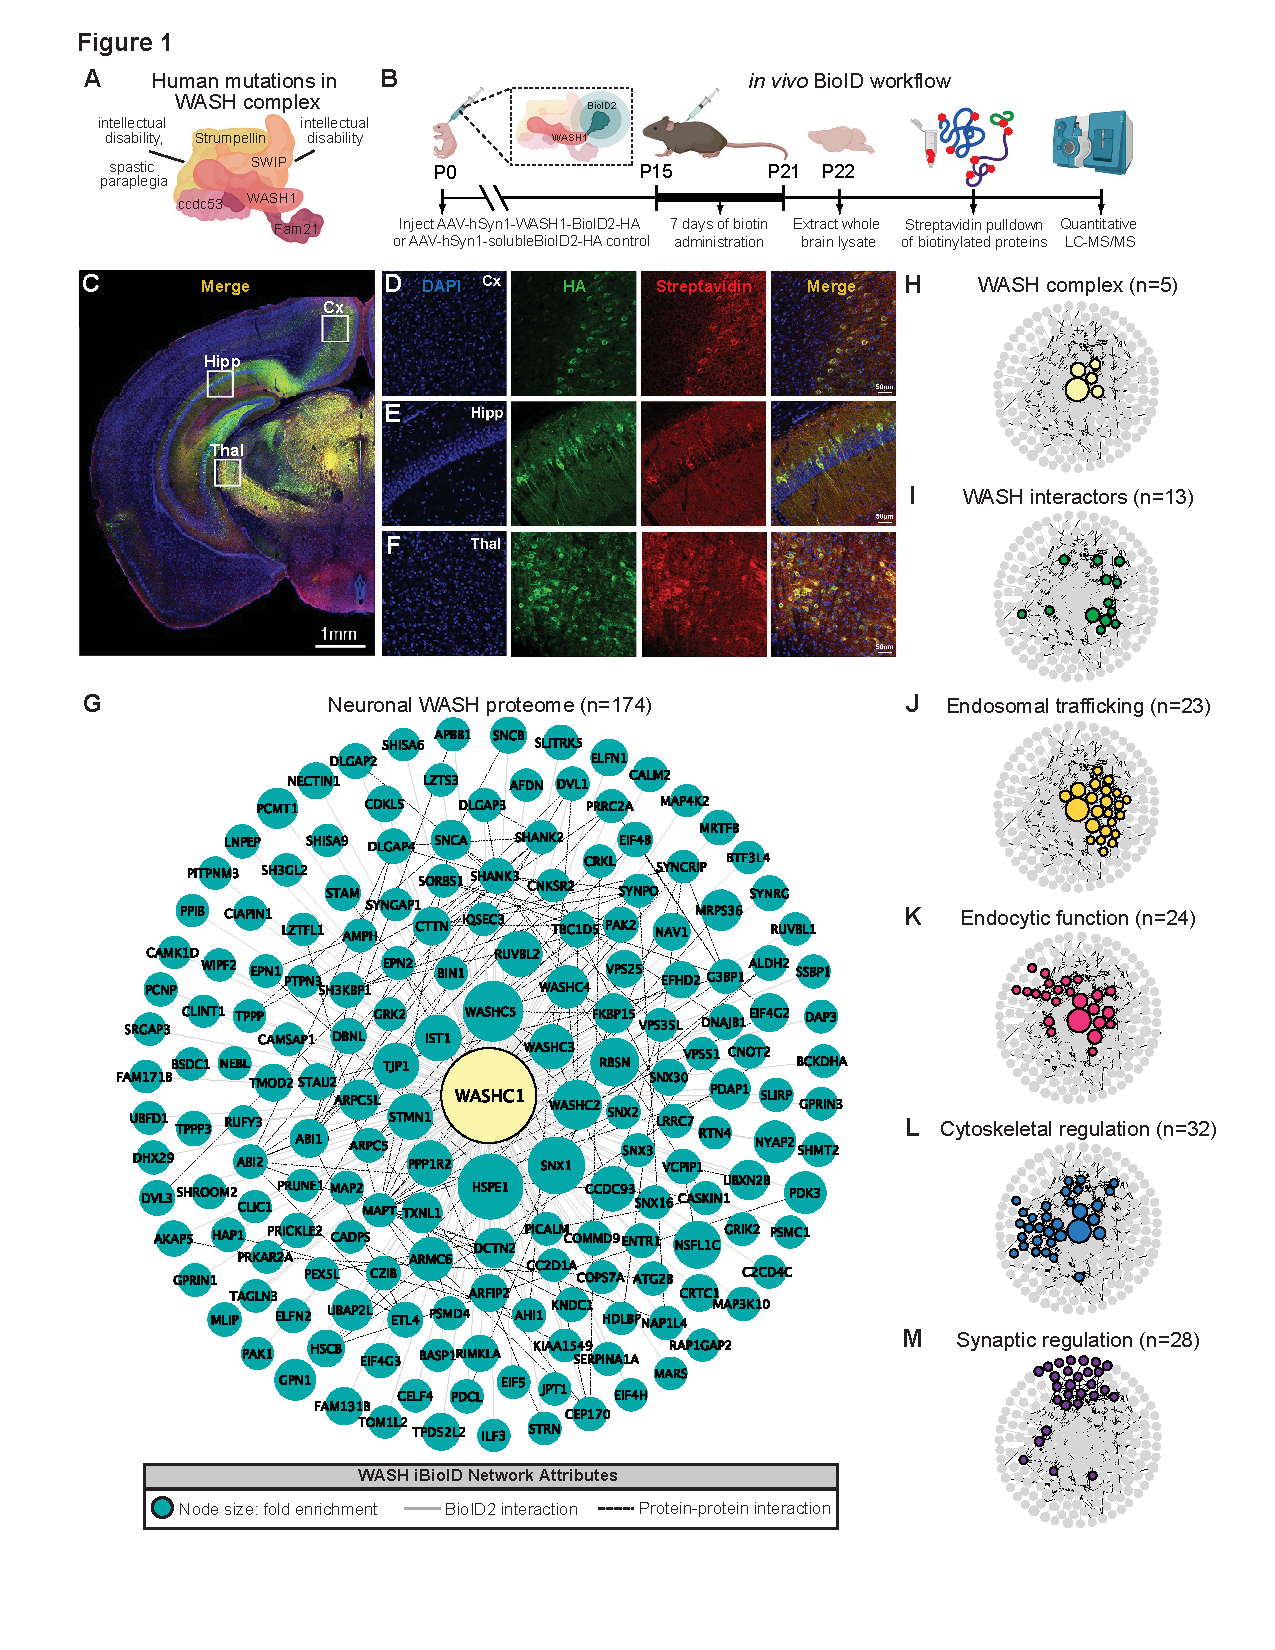
\includegraphics[width=0.95\linewidth, keepaspectratio]{Figure_01}
	\caption{ \textbf{Identification of the WASH complex proteome in vivo confirms a
	neuronal role in endosomal trafficking.}
	(A) The WASH complex is composed of five subunits, Washc1 (WASH1), Washc2
	(FAM21), Washc3 (CCDC53), Washc4 (SWIP), and Washc5 (Strumpellin). Human
	mutations in these components are associated with spastic paraplegia (De Bot et
	al., 2013; Jahic et al., 2015; Valdmanis et al., 2007), Ritscher-Schinzel
	Syndrome (Elliott et al., 2013), and intellectual disability (Assoum et al.,
	2020; Ropers et al., 2011). 
	(B) A BioID2 probe was attached to the c-terminus of WASH1 and expressed under
	the human synapsin-1 (hSyn1) promoter in an AAV construct for in vivo BioID
	(iBioID). iBioID probes (WASH1-BioID2-HA, or negative control solubleBioID2-HA)
	were injected into wild-type mouse brain at P0 and allowed to express for two
	weeks. Subcutaneous biotin injections (24 mg/kg) were administered over seven
	days for biotinylation, and then brains were harvested for isolation and
	purification of biotinylated proteins. LC-MS/MS identified proteins
	significantly enriched in all three replicates of WASH1-BioID2 samples over
	soluble-BioID2 controls. 
	(C) Representative image of WASH1-BioID2-HA expression in a mouse coronal brain
	section (Cx = cortex, Hipp = hippocampus, Thal = thalamus). Scale bar, 1 mm.
	(D) Representative image of WASH1-BioID2-HA expression in mouse cortex (inset
	from C). Individual panels show nuclei (DAPI, blue), AAV construct HA epitope
	(green), and biotinylated proteins (Streptavidin, red). Merged image shows
	colocalization of HA and Streptavidin (yellow). Scale bar, 50 µm. 
	(E) Representative image of WASH1-BioID2-HA expression in mouse hippocampus
	(inset from C). Scale bar, 50 µm.
	(F) Representative image of WASH1-BioID2-HA expression in mouse thalamus (inset
	from C). Scale bar, 50 µm.
	(G) iBioID identified known and unknown proteins interactors of the WASH complex
	in murine neurons. Nodes size represents protein abundance fold-enrichment over
	negative control (range: 3 to 181.7), solid grey edges delineate iBioID
	interactions between the WASHC1 probe (seen in yellow at the center) and
	identified proteins, dashed edges indicate known protein-protein interactions
	from HitPredict database (López et al., 2015). (H-I) Clustergrams of: 
	(H) All five WASH complex proteins identified by iBioID.
	(I) Previously reported WASH interactors (13/174), including the CCC and
	Retriever complexes.
	(J) Endosomal trafficking proteins (23/174 proteins).
	(K) Endocytic proteins (24/174).
	(L) Proteins involved in cytoskeletal regulation (32/174), including Arp2/3
	subunit ARPC5.
	(M) Synaptic proteins (28/174). Clustergrams were annotated by hand and
	cross-referenced with Metascape (Zhou et al., 2019) GO enrichment of WASH1
	proteome constituents over all proteins identified in the BioID experiment.
	}
\label{fig:Figure_01}
\end{fullwidth}
\end{figure}

%-------------------------------------------------------------------------------

The resulting neuronal WASH proteome included 174 proteins that were
significantly enriched (Fold-change $\geq$ 3.0, Benjamini-Hochberg P-Adjust $<$ 0.1,
\textbf{Figure 1G}). Of these proteins, we identified all five WASH complex components
\textbf{(Figure 1H)}, as well as 13 previously reported WASH complex interactors 
\textbf{(Figure 1I)} (McNally et al., 2017; Phillips-Krawczak et al., 2015; Simonetti and
Cullen, 2019; Singla et al., 2019), which provided strong validity for our
proteomic approach and analyses. Additional bioinformatic analyses of the
neuronal WASH proteome identified a network of proteins implicated in vesicular
trafficking, including 23 proteins enriched for endosomal functions \textbf{(Figure 1J)}
and 24 proteins enriched for endocytic functions \textbf{(Figure 1K)}. Among these
endosomal and endocytic proteins were components of the recently identified
endosomal sorting complexes, CCC (CCDC93 and COMMD9) and Retriever (VPS35L)
(Phillips-Krawczak et al., 2015; Singla et al., 2019), as well as multiple
sorting nexins important for recruitment of trafficking regulators to the
endosome and cargo selection, such as SNX1-3, and SNX16 (Kvainickas et al.,
2017; Maruzs et al., 2015; Simonetti et al., 2017). These data demonstrated that
the WASH complex interacts with many of the same proteins in neurons as it does
in yeast, amoebae, flies, and mammalian cell lines. Furthermore, there were 32
proteins enriched for cytoskeletal regulatory functions \textbf{(Figure 1L)}, including
actin-modulatory molecules such as the Arp2/3 complex subunit ARPC5, which is
consistent with WASH’s role in activating this complex to stimulate actin
polymerization at endosomes for vesicular scission (Billadeau et al., 2010;
Derivery et al., 2009). The WASH1-BioID2 isolated complex also contained 28
proteins known to localize to the excitatory post-synapse \textbf{(Figure 1M)}. This
included many core synaptic scaffolding proteins, such as SHANK2-3 and DLGAP2-4
(Chen et al., 2011; Mao et al., 2015; Monteiro and Feng, 2017; Wan et al.,
2011), as well as modulators of synaptic receptors such as SYNGAP1 and SHISA6
(Barnett et al., 2006; Clement et al., 2012; Kim et al., 2003; Klaassen et al.,
2016), which was consistent with the idea that vesicular trafficking plays an
important part in synaptic function and regulation. Taken together, these
results support a major endosomal trafficking role of the WASH complex in mouse
brain. 

\subsection{The SWIP\textsuperscript{P1019R} mutation destabilizes the WASH complex}

To determine how disruption of the WASH complex may lead to
disease, we generated a mouse model of a human missense mutation found in
children with intellectual disability, WASHC4\textsuperscript{c.3056c>g} 
(protein: SWIP\textsuperscript{P1019R}) (Ropers et al., 2011). 
Due to the sequence homology of human and mouse Washc4
genes, we were able to introduce the same point mutation in exon 29 of murine
Washc4 using CRISPR (Derivery and Gautreau, 2010; Ropers et al., 2011). This C>G
point mutation results in a Proline>Arginine substitution at position 1019 of
SWIP’s amino acid sequence \textbf{(Figure 2A)}, a region thought to be critical for its
binding to the WASH component, Strumpellin (Jia et al., 2010; Ropers et al.,
2011). Western blot analysis of brain lysate from adult homozygous SWIP\textsuperscript{P1019R}
mutant mice (referred to from here on as MUT mice) displayed significantly
decreased abundance of two WASH complex members, Strumpellin and WASH1 
\textbf{(Figure 2B)}. These results phenocopied data from the human patients (Ropers et al.,
2011) and suggested that the WASH complex is unstable in the presence of this
SWIP point mutation in vivo. To test whether this mutation disrupted
interactions between WASH complex subunits, we compared the ability of wild-type
SWIP (WT) and SWIP\textsuperscript{P1019R} (MUT) to co-immunoprecipitate with Strumpellin and
WASH1 in HEK cells. Compared to WT, MUT SWIP co-immunoprecipitated significantly
less Strumpellin and WASH1 (IP: 54.8\% and 41.4\% of WT SWIP, respectively),
suggesting that the SWIP\textsuperscript{P1019R} mutation hinders WASH complex formation 
\textbf{(Figure 2 and Figure Supplement 1)}. Together these data support the notion that 
SWIP\textsuperscript{P1019R} is a damaging mutation that not only impairs its function, 
but also results in significant reductions of the WASH complex as a whole.

\subsection{Spatial proteomics analysis of SWIP\textsuperscript{P1019R} mutant mouse brain}

Next, we aimed to understand the impact of the SWIP\textsuperscript{P1019R} mutation on the
subcellular organization of the mouse brain proteome. We performed spatial
proteomics by following the protocol established by Geladaki \textit{et al.}, with
modifications for homogenization of brain tissue (Geladaki et al., 2019; Hallett
et al., 2008). We isolated seven subcellular fractions from brain tissue and
quantified proteins in these samples using 16-plex TMT proteomics. Using this
spatial proteomics dataset, we developed a data-driven clustering approach to
classify proteins into subcellular compartments. This approach, which differs
from the support vector machine learning algorithm employed by Geladaki et al.
(2019), was motivated by the lack of a large corpus of brain-specific protein
subcellular localization information, and the greater complexity of brain tissue
compared to cultured cells. In addition to evaluating differential protein
abundance between WT and SWIP\textsuperscript{P1019R} MUT brain, we utilized this spatial
proteomics dataset to analyze network-level changes in groups of covarying
proteins to better understand WASH’s function and explore the cellular
mechanisms by which SWIP\textsuperscript{P1019R} causes disease. 

Brains from 10-month-old mice were gently homogenized to release intact
organelles, followed by successive centrifugation steps to enrich subcellular
compartments into different fractions based on their density \textbf{(Figure 2C)}
(Geladaki et al., 2019). Seven WT and seven MUT fractions (each prepared from
one brain, 14 samples total) were labeled with unique isobaric tandem-mass tags
and concatenated. We also included two sample pooled quality controls (SPQCs),
which allowed us to assess experimental variability and perform normalization
between experiments. By performing this experiment in triplicate, deep coverage
of the mouse brain proteome was obtained—across all 48 samples we quantified
86,551 peptides, corresponding to 7,488 proteins. After data pre-processing,
normalization, and filtering we retained 5,897 reproducibly quantified proteins
in the final dataset \textbf{(Table S2)}. 

We used generalized linear models (GLMs) to assess differential protein
abundance for intra-fraction comparisons between WT and MUT genotypes, and for
overall comparisons between WT and MUT groups, adjusted for baseline differences
in subcellular fraction. In the first analysis, there were 85 proteins with
significantly altered abundance in at least one of the 7 subcellular fractions
(Benjamini-Hochberg P-Adjust $<$ 0.1, \textbf{Table S2} and 
\textbf{Figure 2 Supplement 2}). Five proteins were differentially abundant 
between WT and MUT in all 7 fractions, including four WASH proteins 
and RAB21A—a known WASH interactor that functions in early endosomal 
trafficking (WASHC1, WASHC2, WASHC4, WASHC5, \textbf{Figure 2E}) 
(Del Olmo et al., 2019; Simpson et al., 2004). The abundance of the
remaining WASH complex protein, WASHC3, was found to be very low and was not
retained in the final dataset due to its sparse quantification. These data
affirm that the SWIP\textsuperscript{P1019R} mutation destabilizes the WASH complex. Next, to
evaluate global differences between WT and MUT brain, we analyzed the average
effect of genotype on protein abundance across all fractions. At this level,
there were 687 differentially abundant proteins between WT and MUT brain
(Bonferroni P-Adjust $<$ 0.05) \textbf{(Table S2)}. We then aimed to place these
differentially abundant proteins into a more meaningful biological context using
a systems-based approach.

For network-based analyses, we clustered the protein covariation network defined
by pairwise correlations between all 5,897 proteins. Our data-driven,
quality-based approach used Network Enhancement (Wang et al., 2018) to remove
biological noise from the covariation network and employed the Leiden algorithm
(Traag et al., 2019) to identify optimal partitions of the graph. We enforced
module quality by permutation testing (Ritchie et al., 2016) to ensure that
identified modules exhibited a non-random topology. Clustering of the protein
covariation graph identified 255 modules of proteins that strongly covaried
together (see Methods for complete description of clustering approach). 
To test for module-level differences between WT and MUT brain, we summarized
modules for each biological replicate (a single subcellular fraction prepared
from either a WT or MUT mouse) as the sum of their proteins, and extended our
GLM framework to identify changes in module abundance (adjusted for fraction
differences) between genotypes. 37 of the 255 modules exhibited significant
differences in WT versus MUT brain (Bonferroni P-Adjust $<$ 0.05; \textbf{Table S3}). 
Of note, the module containing the WASH complex, M19, was predicted to have
endosomal function by annotation of protein function, and was enriched for
proteins identified by WASH1-BioID2 (hypergeometric test P-Adjust $<$ 0.05, bold
node edges, \textbf{Figure 2D}). Similar to the WASH iBioID proteome \textbf{(Figure 1)}, M19
contained components of the CCC (CCDC22, CCDC93, COMMD1-3, COMMD6-7, and COMMD9)
and Retriever sorting complexes (VPS26C and VPS35L), but not the Retromer
sorting complex, suggesting that in the brain, the WASH complex may not interact
as closely with Retromer as it does in other cells \textbf{(Figure 2D)}. Across all
fractions, the abundance of M19 was significantly lower in MUT brain compared to
WT, providing evidence that the SWIP\textsuperscript{P1019R} mutation reduces the stability of
this protein subnetwork and impairs its function \textbf{(Figure 2F-G)}. 

In contrast to the decreased abundance of the WASH complex/endosome module, M19,
we observed three modules (M2, M159, and M213) which were enriched for lysosomal
protein components (Geladaki et al., 2019), and exhibited increased abundance in
MUT brain \textbf{(Figure 3)}. M159 \textbf{(Figure 3B)} contained the lysosomal protease
Cathepsin A (CTSA), while M213 \textbf{(Figure 3D)} contained Cathepsin B (CTSB), as well
as two key lysosomal hydrolases GLB1 and MAN2B2, and M2 \textbf{(Figure 3C)} contained
two Cathepsins (CTSS and CTSL) and several lysosomal hydrolases (e.g. GNS, GLA,
and MAN2B1) (Eng and Desnick, 1994; Mayor et al., 1993; Mok et al., 2003; Moon
et al., 2016; Patel et al., 2018; Regier and Tifft, 1993; Rosenbaum et al.,
2014). Notably, M2 also contained the lysosomal glycoprotein progranulin (GRN),
which is integral to proper lysosome function and whose loss is widely linked
with neurodegenerative pathologies (Baker et al., 2006; Pottier et al., 2016;
Tanaka et al., 2017; Zhou et al., 2018). In addition, M2 contained the hydrolase
IDS, whose loss causes a lysosomal storage disorder that can present with
neurological symptoms (Hopwood et al., 1993; Schröder et al., 1994). The overall
increase in abundance of modules M2, M159, and M213, and these key lysosomal
proteins (Figure 3E-G), may therefore reflect an increase in flux through
degradative lysosomal pathways in SWIP\textsuperscript{P1019R} brain. 

Furthermore, Module 2 \textbf{(Figure 3C)} included multiple membrane proteins and
extracellular proteins, such as ITGA5 (an integrin shown to be upregulated and
redistributed upon loss of WASH1), ATP13A2 (a cation transporter whose loss
causes a Parkinsonian syndrome), and MMP17 (an extracellular metalloprotease),
suggesting a link between these proteins and lysosomal enzymatic function
(English et al., 2000; Ramirez et al., 2006; Zech et al., 2011). Increased
abundance of these M2 proteins in MUT brain may indicate that WASH complex
disruption alters their cellular localization. Taken together, these changes
appear to reflect a pathological condition characterized by distorted lysosomal
metabolism and altered cellular trafficking.

In addition to these endo-lysosomal changes, network alterations were
evident for an endoplasmic reticulum (ER) module (M83), supporting a shift in
the proteostasis of mutant neurons \textbf{(Figure 2 and Figure Supplement 3B)}. Notably,
within the ER module, M83, there was increased abundance of chaperones (e.g.
HSPA5, PDIA3, PDIA4, PDIA6, and DNAJC3) that are commonly engaged in presence of
misfolded proteins (Bartels et al., 2019; Kim et al., 2020; Montibeller and de
Belleroche, 2018; Synofzik et al., 2014; Wang et al., 2016). This elevation of
ER stress modulators can be indicative of neurodegenerative states, in which the
unfolded protein response (UPR) is activated to resolve misfolded species
(Garcia-Huerta et al., 2016; Hetz and Saxena, 2017). These data demonstrate that
loss of WASH function not only alters endo-lysosomal trafficking, but also
causes increased stress on cellular homeostasis. 
Finally, besides these endo-lysosomal and homeostatic changes, we also observed
two synaptic modules (M35 and M248) that were reduced in MUT brain \textbf{(Figure
2 and Figure Supplement 3C-D)}. These included mostly excitatory post-synaptic
proteins such as HOMER2 and DLG4 (also identified in WASH1-BioID, \textbf{Figure 1}),
consistent with endosomal WASH influencing synaptic regulation. Decreased
abundance of these modules indicates that loss of the WASH complex may result in
failure of these proteins to be properly trafficked to the synapse.

\subsection{SWIP mutant neurons display endo-lysosomal structural abnormalities}

Combined, the proteomics data strongly suggested that endo-lysosomal
pathways are altered in adult SWIP\textsuperscript{P1019R} mutant mouse brain. Next, we analyzed
whether structural changes in this system were evident in primary neurons.
Cortical neurons from littermate WT and MUT P0 pups were cultured for 15 days in
vitro (DIV15, Figure 4A), then fixed and stained for established markers of
early endosomes (Early Endosome Antigen 1, EEA1; Figures 4B and 4C) and
lysosomes (Cathepsin D, CathD; Figures 4D and 4E). Reconstructed
three-dimensional volumes of EEA1 and Cathepsin D puncta revealed that MUT
neurons display larger EEA1+ somatic puncta than WT neurons (Figures 4G and 4J),
but no difference in the total number of EEA1+ puncta (Figure 4F). This finding
is consistent with a loss-of-function mutation, as loss of WASH activity
prevents cargo scission from endosomes and leads to cargo accumulation (Bartuzi
et al., 2016; Gomez et al., 2012). Conversely, MUT neurons exhibited
significantly less Cathepsin D+ puncta than WT neurons (Figure 4H), but the
remaining puncta were significantly larger than those of WT neurons (Figures 4I
and 4K). These data support the finding that the SWIP\textsuperscript{P1019R} mutation results in
both molecular and morphological abnormalities in the endo-lysosomal pathway.

\subsection{SWIP\textsuperscript{P1019R} mutant brains exhibit 
lipofuscin accumulation and markers of cell death}

As there is strong evidence that dysfunctional endo-lysosomal trafficking 
and elevated ER stress are associated with neurodegenerative disorders, 
adolescent (P42) and adult (10 month-old, 10mo) WT and MUT brain tissue 
were analyzed for the presence of cleaved caspase-3, a marker of apoptotic 
pathway activation, in four brain regions (Boatright and Salvesen, 2003; 
Porter and Jänicke, 1999). Very little cleaved caspase-3
staining was present in WT and MUT mice at adolescence (Figures 5A, 5B, and
Figure 5-figure supplement 1). However, at 10mo, the MUT motor cortices
displayed significantly greater cleaved caspsase-3 staining compared to
age-matched WT littermate controls (Figures 5D, 5E, and 5H). Furthermore, this
difference appeared to be selective for the motor cortex, as we did not observe
significant differences in cleaved caspase-3 staining at either age for
hippocampal, striatal, or cerebellar regions (Figure 5-figure supplement 1).
These data suggested that neurons of the motor cortex were particularly
susceptible to disruption of endo-lysosomal pathways downstream of SWIP\textsuperscript{P109R},
perhaps because long-range corticospinal projections require high fidelity of
trafficking pathways (Blackstone et al., 2011; Slosarek et al., 2018; Wang et
al., 2014). 

To further examine the morphology of primary motor cortex neurons at a
subcellular resolution, samples from age-matched 7-month-old WT and MUT mice
(7mo, 3 animals each) were imaged by transmission electron microscopy (TEM).
Strikingly, we observed large electron-dense inclusions in the cell bodies of
MUT neurons (arrows, Figure 5L; pseudo-colored region, 5N). These dense
structures were associated electron-lucent lipid-like inclusions (asterisk,
Figure 5N), and were visually consistent with lipofuscin accumulation at
lysosomal residual bodies (Poët et al., 2006; Valdez et al., 2017; Yoshikawa et
al., 2002). Lipofuscin is a by-product of lysosomal breakdown of lipids,
proteins, and carbohydrates, which naturally accumulates over time in
non-dividing cells such as neurons (Höhn and Grune, 2013; Moreno-García et al.,
2018; Terman and Brunk, 1998). However, excessive lipofuscin accumulation is
thought to be detrimental to cellular homeostasis by inhibiting lysosomal
function and promoting oxidative stress, often leading to cell death (Brunk and
Terman, 2002; Powell et al., 2005). As a result, elevated lipofuscin is
considered a biomarker of neurodegenerative disorders, including Alzheimer’s
disease, Parkinson’s disease, and Neuronal Ceroid Lipofuscinoses (Moreno-García
et al., 2018). Therefore, the marked increase in lipofuscin area and number seen
in MUT electron micrographs (Figures 5O and 5P, respectively) is consistent with
the increased abundance of lysosomal pathways observed by proteomics, and likely
reflects an increase in lysosomal breakdown of cellular material. Together these
data indicate that SWIP\textsuperscript{P1019R} results in pathological lysosomal function that
could lead to neurodegeneration. 

\subsection{SWIP\textsuperscript{P1019R} mutant mice display persistent deficits 
in cued fear memory recall}

To observe the functional consequences of the SWIP\textsuperscript{P1019R} mutation, we next
studied WT and MUT mouse behavior. Given that children with homozygous
SWIP\textsuperscript{P1019R} point mutations display intellectual disability (Ropers et al., 2011)
and SWIP\textsuperscript{P1019R} mutant mice exhibit endo-lysosomal disruptions implicated in
neurodegenerative processes, behavior was assessed at two ages: adolescence
(P40-50), and mid-late adulthood (5.5-6.5 mo). Interestingly, MUT mice performed
equivalently to WT mice in episodic and working memory paradigms, including
novel object recognition and Y-maze alternations (Figure 6-figure supplement 1).
However, in a fear conditioning task, MUT mice displayed a significant deficit
in cued fear memory (Figure 6). This task tests the ability of a mouse to
associate an aversive event (a mild electric footshock) with a paired tone
(Figure 6A). Freezing behavior of mice during tone presentation is attributed to
hippocampal or amygdala-based fear memory processes (Goosens and Maren, 2001;
Maren and Holt, 2000; Vazdarjanova and McGaugh, 1998). Forty-eight hours after
exposure to the paired tone and footshock, MUT mice showed a significant
decrease in conditioned freezing to tone presentation compared to their WT
littermates (Figures 6B and 6C). To ensure that this difference was not due to
altered sensory capacities of MUT mice, we measured the startle response of mice
to both electric foot shock and presented tones. In line with intact sensation,
MUT mice responded comparably to WT mice in these tests (Figure 6-figure
supplement 2). These data demonstrate that although MUT mice perceive footshock
sensations and auditory cues, it is their memory of these paired events that is
significantly impaired. Additionally, this deficit in fear response was evident
at both adolescence and adulthood (top panels, and bottom panels, respectively,
Figures 6B and 6C). These changes are consistent with the hypothesis that
SWIP\textsuperscript{P1019R} is the cause of cognitive impairments in humans. 

\subsection{SWIP\textsuperscript{P1019R} mutant mice exhibit surprising motor 
deficits that are confirmed in human patients}

Because SWIP\textsuperscript{P1019R} results in endo-lysosomal pathology
consistent with neurodegenerative disorders in the motor cortex, we next
analyzed motor function of the mice over time. First, we tested the ability of
WT and MUT mice to remain on a rotating rod for five minutes (Rotarod, Figures
7A-7C). At both adolescence and adulthood, MUT mice performed markedly worse
than WT littermate controls (Fig 7C). Mouse performance was not significantly
different across trials, which suggested that this difference in retention time
was not due to progressive fatigue, but more likely due to an overall difference
in motor control (Mann and Chesselet, 2015).

To study the animals’ movement at a finer scale, the gait of WT and MUT mice was
also analyzed using a TreadScan system containing a high-speed camera coupled to
a transparent treadmill (Figure 7D) (Beare et al., 2009). Interestingly, while
the gait parameters of mice were largely indistinguishable across genotypes at
adolescence, a striking difference was seen when the same mice were aged to
adulthood (Figures 7E-7G). In particular, MUT mice took slower (Figure 7E),
longer strides (Figure 7F), stepping closer to the midline of their body (track
width, Figure 7- figure supplement 1), and their gait symmetry was altered so
that their strides were no longer perfectly out of phase (out of phase=0.5,
Figure 7G). While these differences were most pronounced in the rear limbs (as
depicted in Figure 7E-7G), the same trends were present in front limbs (Figure
7-figure supplement 1). These findings demonstrate that SWIP\textsuperscript{P1019R} results in
progressive motor function decline that was detectable by the rotarod task at
adolescence, but which became more prominent with age, as both gait and strength
functions deteriorated.

These marked motor findings prompted us to re-evaluate the original reports of
human SWIP\textsuperscript{P1019R} patients (Ropers et al., 2011). While developmental delay or
learning difficulties were the primary impetus for medical evaluation, all
patients also exhibited motor symptoms (mean age = 10.4 years old, Figure 7H).
The patients’ movements were described as “clumsy” with notable fine motor
difficulties, dysmetria, dysdiadochokinesia, and mild dysarthria on clinical
exam (Figure 7H). Recent communication with the parents of these patients, who
are now an average of 21 years old, revealed no notable symptom exacerbation. It
is therefore possible that the SWIP\textsuperscript{P1019R} mouse model either exhibits
differences from human patients or may predict future disease progression for
these individuals, given that we observed significant worsening at 5-6 months
old in mice (which is thought to be equivalent to ~30-35 years old in humans)
(Dutta and Sengupta, 2016; Zhang et al., 2019).

% Table: Clinical findings in human patients.
%\begin{tabularx}{\textwidth}{X|l}
%\textbf{Patient} & \textbf{Age} & \textbf{Sex} & \textbf{Motor Skills} \\
%\hline
%1 & 18 & F & + \\
%\end{tabularx}

%Figure 2. Spatial proteomics and network covariation analysis reveal significant
%disruptions to the WASH complex and an endosomal module in SWIPP1019R mutant
%mouse brain
%(A) Mouse model of the human SWIPP1019R missense mutation created using CRISPR.
%A C>G point mutation was introduced into exon29 of murine Washc4, leading to a
%P1019R amino acid substitution. We hypothesize (H1) that this mutation causes
%instability of the WASH complex.  
%(B) Representative western blot and quantification of WASH components,
%Strumpellin and WASH1 (predicted sizes in kDa: 134 and 72, respectively), as
%well as loading control β-Tubulin (55kDa) from whole adult whole brain lysate
%prepared from SWIP WT (Washc4C/C) and SWIP homozygous MUT (Washc4G/G) mice.  Bar
%plots show quantification of band intensities relative to WT (n=3 mice per
%genotype). Strumpellin (WT 100.0 ± 5.2%, MUT 3.5 ± 0.7%, t2.1=18.44, p=0.0024)
%and WASH1 (WT 100.0 ± 3.8%, MUT 1.1 ± 0.4%, t2.1=25.92, p=0.0013) were
%significantly decreased. Equivalent amounts of protein were analyzed in each
%condition (β-Tubulin: WT 100.0 ± 8.2%, MUT 94.1 ± 4.1%, U=4, p>0.99). 
%(C) Spatial TMT proteomics experimental design. 7 subcellular fractions were
%prepared from one WT and one MUT mouse (10mo). These samples, as well as two
%pooled quality control (QC) samples, were labeled with unique TMT tags and
%concatenated for simultaneous LC-MS/MS analysis. This experiment was repeated
%three times (3 WT and 3 MUT brains total). To detect network-level changes,
%proteins were clustered into modules, and general linearized models (GLMs) were
%used to identify differences in module abundance between WT and MUT samples. The
%network shows an overview of the spatial proteomics graph in which the 37
%differentially abundant modules are indicated by colored nodes. 
%(D) Protein module 19 (M19) contains subunits of the WASH, CCC, and Retriever
%complexes. Node size denotes its weighted degree centrality (~importance in
%module); purple node color indicates proteins with altered abundance in MUT
%brain relative to WT; black node border denotes proteins identified in the
%WASH1-BioID proteome (Figure 1); red, yellow, and green borders highlight
%protein components of the CCC, Retriever, and WASH complexes; black edges
%indicate known protein-protein interactions; and grey-red edges denote the
%relative strength of protein covariation within a module (gray = weak, red =
%strong). P-adjust values represent enrichment of proteins identified in the
%CORUM database adjusted for multiple comparisons (Giurgiu et al., 2019). 
%(E) Difference in normalized protein abundance for four WASH proteins found in
%M19 (SWIP: WT 6.28 ± 0.41, MUT 4.89 ± 0.28, p=3.98x10-28; WASH1: WT 6.41 ± 0.47,
%MUT 4.65 ± 0.62, p=7.92x10-18; FAM21: WT 6.29 ± 0.48, MUT 5.29 ± 0.49,
%p=3.27x10-16; Strumpellin: WT 7.85 ± 0.52, MUT 6.59 ± 0.53, p=9.06x10-25) and
%one control (Tubulin 4a: WT 8.57 ± 0.52, MUT 8.52 ± 0.58, p>0.99) across all
%three experimental replicates (n=3 independent experiments), presented as
%log2(adjusted protein intensities). 
%(F) Normalized average intensities for every protein within M19 across all seven
%subcellular fractions analyzed. Teal lines delineate protein levels in WT
%samples, purple lines delineate protein levels in MUT samples (averaged across
%three experimental replicates). Bolded lines demarcate the fitted intensity
%values for WT and MUT proteins (n=3 independent experiments). 
%(G) Difference in M19 abundance, adjusted for fraction differences and presented
%as log2(adjusted module abundance) (WT 13.21 ± 0.003, MUT 12.99 ± 0.003,
%p=0.0007; n=3 independent experiments). 
%
%Figure 3. Disruption of lysosomal protein networks in SWIPP1019R mutant brain
%(A) Simplified schematic of the endo-lysosomal pathway in neurons. Inset depicts
%representative lysosomal enzymes, such as proteases (CTSA, CTSB, CTSL),
%glycosidases (GLA, GLB1, MAN2B1), and sulfatases (GNS, IDS).  
%(B) Network graph of module 159 (M159). All proteins in M159 exhibit altered
%abundance in MUT brain, including lysosomal proteins, CTSA, PLA2G15, and GM2A. 
%(C) Module 2 (M2) contains multiple lysosomal proteins with increased abundance
%in MUT brain compared to WT, including CTSS, CTSL, GRN, IDS, MAN2B1. 
%(D) Module 213 (M213) contains multiple proteins with increased abundance in MUT
%brain, including lysosomal proteins, GLB1, GNS, CTSB, MAN2B2, and PLBD2. Network
%attributes (B-D): Node size denotes its weighted degree centrality (~importance
%in module),  node color indicates proteins with altered abundance in MUT brain
%relative to WT, purple outline highlight proteins identified as lysosomal in
%(Geladaki et al., 2019), black edges indicate known protein-protein
%interactions, and grey-red edges denote the relative strength of protein
%covariation within a module (gray = weak, red = strong). P-Adjust values
%represent enrichment of proteins identified as lysosomal in Geladaki et al.,
%2019. 
%(E) The overall effect of genotype on M159 module abundance (WT 10.83 ± 0.002,
%MUT 10.94 ± 0.002, p=0.031). 
%(F) The overall effect of genotype on M2 module abundance (WT 13.74 ± 0.001, MUT
%13.85 ± 0.0009, p=0.0006). 
%(G) The overall effect of genotype on M213 abundance (WT 12.17 ± 0.002, MUT
%12.33 ± 0.002, p=0.0037). Data reported as mean ± SEM, error bars are SEM.
%*p<0.05, ** p<0.01, ***p<0.001, empirical Bayes quasi-likelihood F-test with
%Bonferroni correction (E-G).
%
%Figure 4. SWIPP1019R mutant neurons display structural abnormalities in
%endo-lysosomal compartments in vitro 
%(A) Experimental design. Cortices were dissected from P0 pups, and neurons were
%dissociated and cultured on glass coverslips for 15 days. Cultures were fixed,
%stained, and imaged using confocal microscopy. 3D puncta volumes were
%reconstructed from z-stack images using Imaris software. 
%(B-C) Representative 3D reconstructions of WT and MUT DIV15 neurons
%(respectively) stained for EEA1 (yellow) and MAP2 (magenta). 
%(D-E) Representative 3D reconstructions of WT and MUT DIV15 neurons
%(respectively) stained for Cathepsin D (cyan) and MAP2 (magenta). 
%(F) Graph of the average number of EEA1+ volumes per soma in each image (WT 95.0
%± 5.5, n=24 neurons; MUT 103.7 ± 3.7, n=24 neurons; t40.2=1.314, p=0.1961). 
%(G) Graph of the average EEA1+ volume size per soma shows larger EEA1+ volumes
%in MUT neurons (WT 0.15 ± 0.01 µm3, n=24 neurons; MUT 0.30 ± 0.02 µm3, n=24
%neurons; U=50, p<0.0001). 
%(H) Graph of the average number of Cathepsin D+ volumes per soma illustrates
%less Cathepsin D+ volumes in MUT neurons (WT 30.4 ± 1.4, n=42; MUT 17.2 ± 0.9,
%n=42; t71=7.943, p<0.0001). 
%(I) Graph of the average Cathepsin D+ volume size per soma demonstrates larger
%Cathepsin D+ volumes in MUT neurons (WT 0.54 ± 0.02 µm3, n=42; MUT 0.69 ± 0.04
%µm3, n=42; t63=3.701, p=0.0005). 
%(J) Histogram of EEA1+ volumes illustrate differences in size distributions
%between MUT and WT neurons. 
%(K) Histogram of CathD+ volumes show differences in size distributions between
%MUT and WT neurons. Analyses included at least three separate culture
%preparations. Scale bars, 5 µm (B-E). Data reported as mean ± SEM, error bars
%are SEM. ***p<0.001, ****p<0.0001, two-tailed t-tests or Mann-Whitney U test
%(G).
%
%Figure 5. SWIPP1019R mutant brains exhibit markers of abnormal endo-lysosomal
%structures and cell death in vivo
%(A-B) Representative images of adolescent (P42) WT and MUT motor cortex stained
%with cleaved caspase-3 (CC3, green).
%(C) Anatomical representation of mouse brain with motor cortex highlighted in
%red, adapted from the Allen Brain Atlas (Oh et al., 2014). 
%(D-E) Representative image of adult (10 mo) WT and MUT motor cortex stained with
%CC3 (green).  
%(F, G, I, and J) DAPI co-stained images for (A, B, D, and E, respectively).
%Scale bar for (A-J), 15 µm. 
%(H) Graph depicting the normalized percentage of DAPI+ nuclei that are positive
%for CC3 per image. No difference is seen at P42, but the amount of CC3+ nuclei
%is significantly higher in aged MUT mice (P42 WT 6.97 ± 0.80%, P42 MUT 5.26 ±
%0.90%, 10mo WT 25.38 ± 2.05%, 10mo MUT 44.01 ± 1.90%, H=74.12, p<0.0001). We
%observed no difference in number of nuclei per image between genotypes. 
%(K) Representative transmission electron microscopy (TEM) image taken of soma
%from adult (7mo) WT motor cortex. Arrowheads delineate electron-dense lipofuscin
%material, Nuc = nucleus. 
%(L) Representative transmission electron microscopy (TEM) image taken of soma
%from adult (7mo) MUT motor cortex. 
%(M) Inset from (K) highlights lysosomal structure in WT soma. Pseudo-colored
%region depicts lipofuscin area, demarcated as L. 
%(N) Inset from (L) highlights large lipofuscin deposit in MUT soma (L,
%pseudo-colored region) with electron-dense and electron-lucent lipid-like
%(asterisk) components. 
%(O) Graph of areas of electron-dense regions of interest (ROI) shows increased
%ROI size in MUT neurons (WT 2.4x105 ± 2.8x104 nm2, n=50 ROIs; MUT 8.2x105 ± 9.7
%x104 nm2, n=75 ROIs; U=636, p<0.0001). 
%(P) Graph of the average number of presumptive lysosomes with associated
%electron-dense material reveals increased number in MUT samples (WT 3.14 ± 0.72
%ROIs, n=14 images; MUT 10.86 ± 1.42 ROIs, n=14 images; U=17, p<0.0001). For (N)
%and (O), images were taken from multiple TEM grids, prepared from n=3 animals
%per genotype. Scale bar for all TEM images, 1 µm. Data reported as mean ± SEM,
%error bars are SEM. ***p<0.001, ****p<0.0001, Kruskal-Wallis test (F),
%Mann-Whitney U test (O-P).
%
%Figure 6. SWIPP1019R mutant mice display persistent deficits in cued fear memory
%recall 
%(A) Experimental fear conditioning paradigm. After acclimation to a conditioning
%chamber, mice received a mild aversive 0.4mA footshock paired with a 2900Hz
%tone. 48 hours later, the mice were placed in a chamber with different tactile
%and visual cues. The mice acclimated for two minutes and then the 2900Hz tone
%was played (no footshock) and freezing behavior was assessed. 
%(B) Line graphs of WT and MUT freezing response during cued tone memory recall.
%Data represented as average freezing per genotype in 30 s time bins. The tone is
%presented after t = 120 s, and remains on for 120 seconds (Tone ON). Two
%different cohorts of mice were used for age groups P42 (top) and 6.5mo (bottom).
%Two-way ANOVA analysis of average freezing during Pre-Tone and Tone periods
%reveal a Genotype x Time effect at P42 (WT n=10, MUT n=10, F1,18=4.944,
%p=0.0392) and 6.5mo (WT n=13, MUT n=11, F1,22= 13.61, p=0.0013). 
%(C) Graphs showing the average %time freezing per animal before and during tone
%presentation. Top: freezing is reduced by 20% in MUT adolescent mice compared to
%WT littermates (Pre-tone WT 16.5 ± 2.2%, n=10; Pre-tone MUT 13.0 ± 1.8%, n=10;
%t36=0.8569, p=0.6366; Tone WT 52.8 ± 3.8%, n=10; Tone MUT 38.0 ± 3.6%, n=10;
%t36=3.539, p=0.0023), Bottom: freezing is reduced by over 30% in MUT adult mice
%compared to WT littermates (Pre-tone WT 21.1 ± 2.7%, n=13; Pre-tone MUT 23.7 ±
%3.8%, n=11; t44=0.4675, p=0.8721; Tone WT 69.7 ± 4.3%, n=13; Tone MUT 53.1 ±
%5.2%, n=11; t44=2.921, p=0.0109). Data reported as mean ± SEM, error bars are
%SEM. *p<0.05, **p<0.01, two-way ANOVAs (B) and Sidak’s post-hoc analyses (C).
%
%Figure 7. SWIPP1019R mutant mice exhibit surprising motor deficits that are
%confirmed in human patients 
%(A) Rotarod experimental setup. Mice walked atop a rod rotating at 32rpm for 5
%minutes, and the duration of time they remained on the rod before falling was
%recorded. 
%(B) Line graph of average duration animals remained on the rod per genotype
%across four trials, with an inter-trial interval of 40 minutes. The same cohort
%of animals was tested at two different ages, P45 (top) and 5.5 months (bottom).
%Genotype had a significant effect on task performance at both ages (top, P45:
%genotype effect, F1,25=7.821, p=0.0098. bottom, 5.5mo: genotype effect, F1,23=
%7.573, p=0.0114). 
%(C) Graphs showing the average duration each animal remained on the rod across
%trials. At both ages, the MUT mice exhibited an almost 50% reduction in their
%ability to remain on the rod (Top, P45: WT 169.9 ± 25.7 s, MUT 83.8 ± 15.9 s,
%U=35, p=0.0054. Bottom, 5.5mo: WT 135.9 ± 20.9 s, MUT 66.7 ± 9.5 s, t18=3.011,
%p=0.0075). 
%(D) TreadScan task. Mice walked on a treadmill for 20 s while their gate was
%captured with a high-speed camera. Diagrams of gait parameters measured in (E-G)
%are shown below the TreadScan apparatus. 
%(E) Average swing time per stride for hindlimbs. At P45 (top), there is no
%significant difference in rear swing time (WT 156.2 ± 22.4 ms, MUT 132.3 ± 19.6
%ms, U=83, p=0.7203). At 5.5mo (bottom), MUT mice display significantly longer
%rear swing time (WT 140 ± 6.2 ms, MUT 252.0 ± 21.6 ms, t12=4.988, p=0.0003). 
%(F) Average stride length for hindlimbs. At P45 (top), there is no significant
%difference in stride length (WT 62.3 ± 2.0 mm, MUT 60.5 ± 2.1 mm, U=75,
%p=0.4583). At 5.5mo (bottom), MUT mice take significantly longer strides with
%their hindlimbs (WT 60.8 ± 0.8 mm, MUT 73.6 ± 2.7 mm, t11.7=4.547, p=0.0007). 
%(G) Average homologous coupling for front and rear limbs. Homologous coupling is
%0.5 when the left and right feet are completely out of phase. At P45 (top), WT
%and MUT mice exhibit normal homologous coupling (WT 0.48 ± 0.005, MUT 0.48 ±
%0.004, U=76.5, p=0.4920). At 5.5 mo (bottom), MUT mice display decreased
%homologous coupling, suggestive of abnormal gait symmetry (WT 0.48 ± 0.003, MUT
%0.46 ± 0.004, t18.8=3.715, p=0.0015). At P45: n=14 WT, n=13 MUT; At 5.5mo: n=14
%WT, n=11 MUT. 
%(H) Table of motor findings in clinical exam of human patients with the
%homozygous SWIPP1019R mutation. All patients exhibit motor dysfunction (+ =
%symptom present). Data reported as mean ± SEM, error bars are SEM. *p<0.05,
%**p<0.01, ***p<0.001, ****p<0.0001, two-way repeated measure ANOVAs (B),
%Mann-Whitney U tests and two-tailed t-tests (C-G).

%Figure 8. Model of neuronal endo-lysosomal pathology in SWIPP1019R mutant mice
%(A) Wild-type WASH function in mouse brain. Under normal conditions, the WASH
%complex interacts with many endosomal proteins and cytoskeletal regulators, such
%as the Arp2/3 complex. These interactions enable restructuring of the endosome
%surface (actin in gray) and allow for cargo segregation and scission of
%vesicles. Substrates are transported to the late endosome for lysosomal
%degradation, to the Golgi network for modification, or to the cell surface for
%recycling. 
%(B) Loss of WASH function leads to increased lysosomal degradation in mouse
%brain. Destabilization of the WASH complex leads to enlarged endosomes and
%lysosomes, with increased substrate accumulation at the lysosome. This suggests
%an increase in flux through the endo-lysosomal pathway, possibly as a result of
%mis-localized endosomal substrates. 
%(C) Wild-type mice exhibit normal motor function. 
%(D) SWIPP1019R mutant mice display progressive motor dysfunction in association
%with these subcellular alterations.
